%!TEX root = ../../../../report.tex

\subsection{Ankle and knee joint mechanics} % (fold)
\label{sub:hip_and_knee_joint_mechanics}

\subsubsection{Rods} % (fold)
\label{ssub:rods}
As explained in section \ref{sub:bearings}, it was decided to have two bearings per link (which gives four per joint) and a rod going through them.
This rod is then also used, in the case of the knee and the ankle, as a support for the pulleys that transmit the power from the motor to the next link.

Three mechanical efforts bound its design:
\begin{enumerate}
  \item \textbf{Shear strength}: in the case of the shear produced when an impact occurs and the rod of one link moves in the opposite direction than its relative in the consecutive link.
  \item \textbf{Resistance to bending}: due to the bending effort that the tension of the belt is constantly applying in the rod of the  knee and the ankle.
  \item \textbf{Torsion}: due to the pulley in the knee and the ankle. 
  This effort is negligible because zero-friction bearings are supposed.
\end{enumerate}

  \paragraph{Shear analysis} % (fold)
  \label{ssub:shear_analysis}
  The maximum shear stress is found in the diameter of the cylinder (y=0) and is:
  
  \noindent\begin{minipage}{0.2\textwidth}% adapt widths of minipages to your needs
  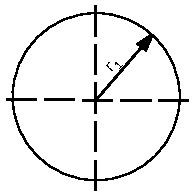
\includegraphics[width=\linewidth]{figures/profile_tube.pdf}
  \end{minipage}%
  \hfill%
  \begin{minipage}{0.8\textwidth}
    \begin{equation}
    \begin{aligned}
      \gamma_{yz} &= \frac{Q_y M_{x}^A*}{b(y) I_x} = \frac{Q}{r^2}\\
      M_{x}^{A_{y=0}} &= \frac{\pi r_1^2}{2} \\
      b(y=0) &= 2 r_1 \\
      I_x &= \frac{\pi r_1^4}{4}
      \end{aligned}
    \end{equation}
  \end{minipage}
  Given a tangent force Q, the shear stress can be calculated.
  If this is over the ultimate strength, the cylinder will break.
  % paragraph shear_analysis (end)

  \paragraph{Bending} % (fold)
  \label{ssub:bending}
  The bending analysis follows the one carried out in the section \ref{ssub:profile_study} for a cylinder.
  The equivalent force in this case is given by the tension of the belts, mainly the initial (though there are other tensions that appear when the belts moves for example).
  Due to feasibility reasons and the lack of the appropriate measurements devices, some experimental tests trying different tensions and axes where carried out giving good results with a 3 mm rod or more.
  % paragraph bending (end)

  \paragraph{Sizing} % (fold)
  \label{ssub:sizing}
  The studies above have been tested for different diameters of rod starting from the smallest size given by the provider and increasing until both conditions are satisfied, due to the requirements of weight reduction.
  In case of using steel as material, the ultimate strength is supposed to be 250 MPa \footnote{https://en.wikipedia.org/wiki/A36\_steel}.
  And for the case of a rod of 3 mm of diameter, both stresses are under the restrictions.
  Thus, 3 mm rods are going to be used.
  % paragraph sizing (end)
% subsubsection rods (end)

\subsubsection{Bearings} % (fold)
\label{ssub:bearings}
In the section \ref{sub:impact_force} the force for sizing the bearings of the knee and the ankle was calculated.
The bearing elected would be such that allows dynamic loads of more than the impact force while keeping as small as possible to reduce the added weight to the robot.
On the other hand, the internal diameter comes defined by the rod diameter calculated in the section \ref{sub:rods}.

An estimation of nominal life of the bearing can be done from the Dynamic Load Rating (C), the Dynamic Equivalent Load (P) and the Life Rime Coefficient for a Ball Bearing (p) (being p=3 for balls bearings).
The equation \ref{eq:service_life_bearing}, shows the nominal life of a ball bearing that can be used in order to calculate the nominal life for a specific application.
It is also worth to mention that the Dynamic Equivalent Load (P) is divided by the number of bearings in which the force is spread.
\begin{equation}
  \label{eq:service_life_bearing}
  L_{10} = \frac{10^{6}}{60 n} \left(\frac{C}{P}\right)^{p}
\end{equation}

The term $L$ is the service life of a bearing (in number of hours or rpm), in normal conditions of speed and load, in which the bearing is working until fail by fatigue. 
Whilst $L_{10}$ is based in a stadistical model that is defined as the 90\% of the bearing of the same type will withstand those loads for a longer time.
% subsubsection bearings (end)

\subsubsection{Spring integration} % (fold)

\todo{Springs selection (shortly)}

\label{ssub:spring_integration}
In the section \ref{sub:compliance}, is justified the use of springs in order to walk and run efficiently. 
Later, an extensive analysis of the different possibilities to include compliance in the robot is done in the same section.
The Figure \ref{fig:compliance_series} shows the analyzed configurations and their advantages and disadvantages are further discussed.
Due to the role that RuBi takes inside of the project, it is decided that all the configurations can be taken.
This is possible by making a system that allows to put elastic components in series and parallel that are easily replaceable.
Furthermore, a big range of springs have been ordered for the reasons in explained in \ref{sec_springs}.
All the springs can be placed due to the hole for inserting the springs has the diameter of the biggest one ordered plus a small clearance obtained from \ref{sub:arc_compensation}.

\paragraph{SEA configuration} % (fold)
\label{para:sea_configuration}

In the section commented above, it is also determined the use of rotational springs for both series and parallel passive actuators.
This gives a more constrained design that is later used as a feature.
For example, in the section \ref{sub:pulleys_and_belts} is explained how the the pulley is integrated in a part that has the task of both being the place to put the spring and being the pulley.
The Figure \ref{fig:serial_spring_pulley} shows this design.
This design shows the implementation of the SEA configurations that can be adjusted by changing the physical properties of the spring.
% paragraph sea_configuration (end)

\paragraph{PEA configuration} % (fold)
\label{para:pea_configuration}

The parallel spring is implemented by adding a spring directly attached to both parts of the joint.
The problem of the parallel passive actuators is the need of loading the spring for movements in which is maybe not appropriated.
As an example, the rest position of the parallel spring in the ankle could to be placed when the foot is at 90 degrees with its consecutive link, so the robot can be stood up without applying any extra torque in the motors to keep balance.
This would mean though to do an extra effort against the spring when taking off.

In the same line of giving all the possibilities to the user with the compliance, a system that allows to change the rest position of the parallel spring has been implemented.
This consists of one arm of the torsional spring attached to one of the links of the joint while the other arm can be fastened in different positions.
The Figure \ref{fig:rotational_spring_rest_position} shows the transversal section of the part where the parallel spring can adopt different configurations. 
This gives the different PEA configurations by just changing the physical properties of the spring and by using a spring stiff enough in the SEA that would act as DD.

\begin{figure}[ht!]
  \centering
  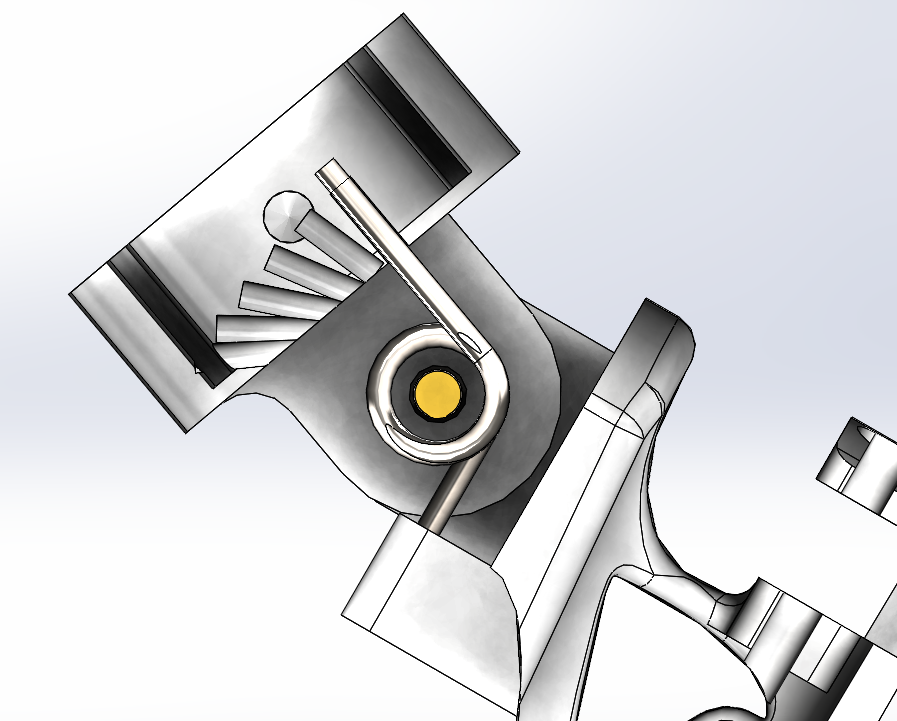
\includegraphics[width=0.75\textwidth]{figures/rotational_spring_rest_positions}
  \caption{Transversal section of the parallel spring resting positions in the left ankle.}
  \label{fig:rotational_spring_rest_position}
\end{figure}
% paragraph pea_configuration (end)

\paragraph{SEA + PEA configuration} % (fold)
\label{ssub:sea_pea_configuration}
The possibility of using both, SEA and PEA, configurations at the same time is given.
This lets the study of the combination of both configuration.
% paragraph sea_pea_configuration (end)

\paragraph{DD configuration } % (fold)
\label{ssub:dd_configuration}
Finally if no parallel spring is used and a spring stiff enough that doesn't add compliance to the system is placed, a DD configuration is achieved.
% paragraph dd_configuration (end)

% subsubsection spring_integration (end)

% subsection hip_and_knee_joint_mechanics (end)
